%
% 6.006 problem set 3 solutions template
%
\documentclass[12pt,twoside]{article}

\input{macros-sp20}
\newcommand{\theproblemsetnum}{3}

\title{6.006 Problem Set \theproblemsetnum}

\begin{document}

\handout{Problem Set \theproblemsetnum}

\setlength{\parindent}{0pt}
\medskip\hrulefill\medskip

{\bf Name:} Your Name

\medskip

{\bf Collaborators:} Name1, Name2

\medskip\hrulefill

%%%%%%%%%%%%%%%%%%%%%%%%%%%%%%%%%%%%%%%%%%%%%%%%%%%%%
% See below for common and useful latex constructs. %
%%%%%%%%%%%%%%%%%%%%%%%%%%%%%%%%%%%%%%%%%%%%%%%%%%%%%

% Some useful commands:
%$f(x) = \Theta(x)$
%$T(x, y) \leq \log(x) + 2^y + \binom{2n}{n}$
% {\tt code\_function}


% You can create unnumbered lists as follows:
%\begin{itemize}
%    \item First item in a list
%        \begin{itemize}
%            \item First item in a list
%                \begin{itemize}
%                    \item First item in a list
%                    \item Second item in a list
%                \end{itemize}
%            \item Second item in a list
%        \end{itemize}
%    \item Second item in a list
%\end{itemize}

% You can create numbered lists as follows:
%\begin{enumerate}
%    \item First item in a list
%    \item Second item in a list
%    \item Third item in a list
%\end{enumerate}

% You can write aligned equations as follows:
%\begin{align}
%    \begin{split}
%        (x+y)^3 &= (x+y)^2(x+y) \\
%                &= (x^2+2xy+y^2)(x+y) \\
%                &= (x^3+2x^2y+xy^2) + (x^2y+2xy^2+y^3) \\
%                &= x^3+3x^2y+3xy^2+y^3
%    \end{split}
%\end{align}

% You can create grids/matrices as follows:
%\begin{align}
%    A =
%    \begin{bmatrix}
%        A_{11} & A_{21} \\
%        A_{21} & A_{22}
%    \end{bmatrix}
%\end{align}

% You can include images and PDFs as follows:
% \includegraphics[width=0.5\textwidth]{img.jpg}

\begin{problems}

\problem  % Problem 1

\begin{problemparts}
\problempart % Problem 1a
Known: $h(k)=(10k+4)$ mod 7

$h(47)=5, h(61)=5,h(36)=0,h(52)=6,h(56)=4,h(33)=5,h(92)=0$

\begin{center}
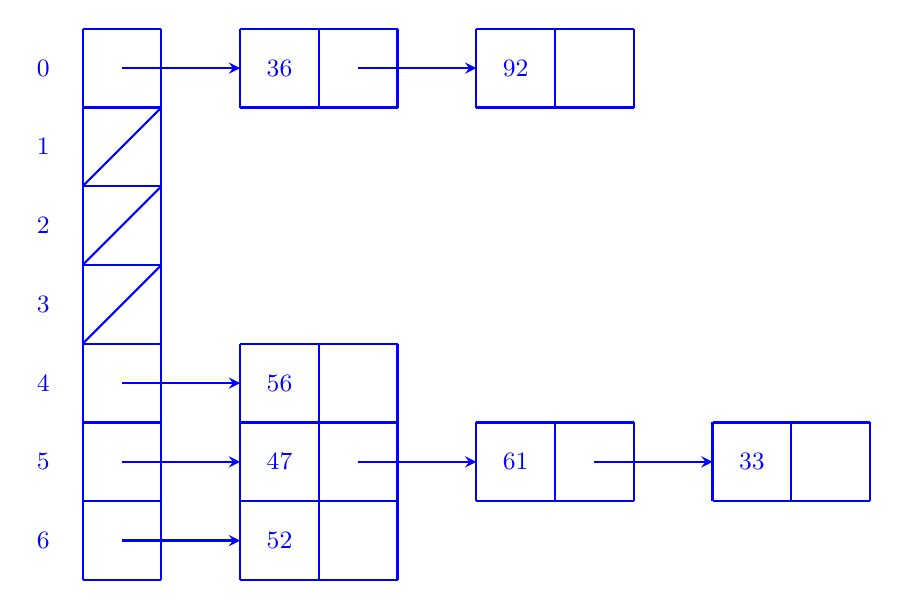
\begin{tikzpicture}[font=\small,thick,>=stealth, color=blue]
    \foreach \j in {1,2,3}{
       \draw (1,-\j)--+(-1,-1); % 从 (1, -j) 划线到 (1 - 1, - j - 1)
    }
    \draw (0,0) grid (1,-7);
    \foreach \i in {0,...,6}{
       \path (-0.5,-\i-0.5) node{$ \i $};   % 分别是左上角右下角左边
    }
     \foreach \i/\j in {0/36,4/56,5/47,6/52}{
       \draw[->] (0.5,-\i-0.5)--+(1.5,0)    % 从 (0.5, -i - 0.5) 划线到 (2, - i - 1.5)
       node[shift={(0.5,0)}]{$ \j $};
       \draw (2,-\i - 0) grid +(2,-1);
     }
     \foreach \i/\j in {0.5/92,5.5/61}{
       \draw[->] (3.5,-\i)--+(1.5,0) node[shift={(0.5,0)}]{$ \j $};
     }
     \draw[->] (6.5,-5.5)--+(1.5,0) node[shift={(0.5,0)}]{$ 33 $};
     \draw (5,0) grid +(2,-1) (5,-5) grid +(2,-1) (8,-5) grid +(2,-1);
\end{tikzpicture}
\end{center}

\newpage
\problempart % Problem 1b
Known: $h(k)=((10k+4)$ mod c) mod 7
\begin{lstlisting}
def main():
    data = [47, 61, 36, 52, 56, 33, 92]
    'In python, set and dictionary are both based on hash table.'
    record = set()
    for c in range(1, 100):
        flag = True
        for a in data:
            x = ((10 * a + 4) % c) % 7
            if x in record:
                flag = False
                break
            record.add(x)
        if flag:
            print(c)
            break
        record.clear()

if __name__ == '__main__':
    main()
\end{lstlisting}
Answer is 13, then there is no collision.

\end{problemparts}

\problem  % Problem 2

\begin{problemparts}
\problempart % Problem 2a
Known: $H = \{h_{ab}(k) = (ak + b)\;mod\;n\;|\;a, b \in  \{0,...,n-1\}\;and\;a\ne0\}$
$$
\exists k_1,k_2, h(k1)=h(k2)\Leftrightarrow ak_1+b\equiv ak_2+b(mod\;n)
\Leftrightarrow a(k_1-k_2)\equiv 0(mod\;n),\forall a \in \mathbb{Z} 
\Leftrightarrow n | (k_1-k_2)
$$

\problempart % Problem 2b
$n\;|\;(\lfloor\frac{k_1n}{u})\rfloor-\lfloor\frac{k_2n}{u}\rfloor$

But $k_1,k_2<u\Rightarrow \lfloor\frac{k_{1(2)}n}{u}\rfloor<n$, we can deduce that
the difference must be 0: $\lfloor\frac{k_1n}{u}\rfloor=\lfloor\frac{k_2n}{u}\rfloor$.

We can take $k_1=1,k_2=2$ because then $\frac{u}{k_{1(2)}}\gg n$
$\Rightarrow \lfloor\frac{k_1n}{u}\rfloor=\lfloor\frac{k_2n}{u}\rfloor=0$

\problempart % Problem 2c
Seen the cour: the probability maximum is $\frac{1}{m}$

\end{problemparts}

\newpage

\problem  % Problem 3

\begin{problemparts}
\problempart % Problem 3a
Use \textbf{radix sort}: a string is divided into multiple ASCII characters, which can be
described by a number from 0 to 127. The length of string is fixed. So we can get
the time: $\Theta(nlog_4n)$. In a comparative model, each comparison of string will
cost extra $\Theta(log_4n)$ time, which leads to the time total: $O(nlog^2n)$

\problempart % Problem 3b
\begin{enumerate}
    \item $n \gg 800,000$, then
    $800,000$ is not a big number, so we can use \textbf{count sort}. The space cost will depend 
    on $n$. The time cost $\Theta(n+800,000)\simeq \Theta(n)$
    \item Otherwise, we can use merge sort et etc.
\end{enumerate}

\problempart % Problem 3c
Multiply by $n^3$, then use radix sort: $\Theta(n)$

\problempart % Problem 3d
This is a comparative model, where we can use merge sort: $\Theta(nlogn)$

\end{problemparts}

\problem  % Problem 4

\begin{problemparts}
\problempart % Problem 4a
Use a hash table to store $(i, r - b_i)$ pair.

\problempart % Problem 4b
\end{problemparts}

\problem  % Problem 5

\begin{problemparts}
\problempart % Problem 5a
Use hash table. For a string A, we extract a substring of which length is k. We sort it
by using bucket sort: $\Theta(k+26)\simeq \Theta(k)$. The result of sort is the key of 
hash table. The value is a index sort.

When we search the anagram substring count of B, we just ust bucket sort to sort B at first
and then return the size of $h(key)$

\problempart % Problem 5b
Use the method of problem above is fine.
\begin{lstlisting}
def count_anagram_substrings(T, S):
    '''
    Input:  T | String
            S | Tuple of strings S_i of equal length k < |T|
    Output: A | Tuple of integers a_i:
              | the anagram substring count of S_i in T
    '''
    A = []
    ##################
    # YOUR CODE HERE #
    ##################
    k = len(S[0])
    record = {}
    for i in range(0, len(T) - k + 1):
        R = bucket_sort(T[i:i + k])
        if R not in record:
            record[R] = 1
        else:
            record[R] += 1
    for s in S:
        R = bucket_sort(s)
        if R in record:
            A.append(record[R])
        else:
            A.append(0)
    return tuple(A)

def bucket_sort(T):
    A = [0] * 26
    for t in T:
        A[ord(t) - 97] += 1
    S = ""
    for i in range(26):
        S += chr(i + 97) * A[i]
    return S
\end{lstlisting}
\textcolor{red}{Solution is basiclly same as mine. But there is no need to calculate R each time,
we can use a window of size 26.}


\problempart Submit your implementation to {\small\url{alg.mit.edu}}.
\end{problemparts}

\end{problems}

\end{document}
